\part{Connect Database}

\begin{frame}{Local Development Environment Setup}
\textbf{Principle:} Setup development environment as similar as possible as on Cloud Foundry
\vfill
Configure system environment variables to connect to 
\begin{enumerate}
\item Locally installed services
\item Cloud Foundry services via \colorlink{https://github.infra.hana.ondemand.com/cloudfoundry/chisel}{Chisel} tunnel, \codealt{cf local} (\colorlink{https://github.wdf.sap.corp/xs2/cflocal-plugin}{Plugin}) or \colorlink{https://blogs.sap.com/2018/04/27/how-to-use-an-ssh-tunnel-with-scp-cloud-foundry-backing-service/}{SSH} tunnel
\end{enumerate}
\vfill
\includeGraphicsLocalEnvironmentSetup{width=1.0\textwidth}
\end{frame}

\begin{frame}{Exercise 7}
\colorlink{https://github.com/ccjavadev/cc-coursematerial/blob/master/ConnectDatabase/Exercise_7_ConnectLocalDatabase.md}{Exercise 7: Setup local environment with database connection}
\end{frame}

\begin{frame}[fragile]{JPA: Java Persistence API}{Persist objects into database}
JPA
\begin{itemize}
\item O-R mapping: Maps objects to relational databases like PostgreSQL
\item Common JPA implementations: \colorlink{http://www.eclipse.org/eclipselink/}{\underline{EclipseLink}} and \colorlink{http://hibernate.org/orm/}{Hibernate}
\end{itemize}

\visible<2->{
Entity %long-lives and survives both a crash or a shutdown of the server
\begin{itemize}
\item represents a business object like Customer or Order 
\item is a Java class annotated with \codealt{@Entity}
\item has a primary key using \codealt{@Id} annotation
\end{itemize}
}

\visible<3->{
Entity Manager
\begin{itemize}
\item records activities on the managed entities within transaction
\item translates CRUD operations to SQL just before commit
\end{itemize}
}

\end{frame}

\begin{frame}[fragile]{JPA: Entity example}
\begin{columns}
	\begin{column}[T]{.5\textwidth}	
		Declaration:
\begin{lstlisting}
@Entity
class User {
    @Id
    private Long id;

    private String city;

    @OneToMany
    private Collection<Account> accounts;
}
\end{lstlisting}
	\end{column}
	\begin{column}[T]{.45\textwidth}	
		\begin{figure}
	  		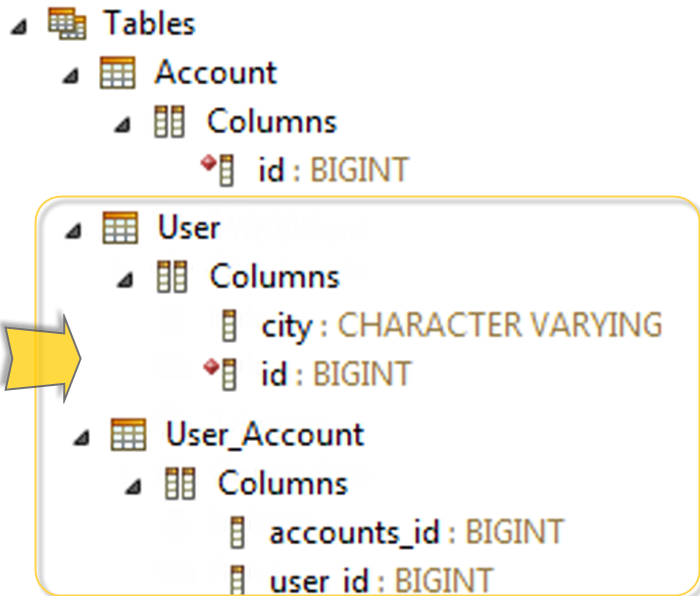
\includegraphics[width=0.9\textwidth]{../ConnectDatabase/images/EntityTables}
		\end{figure}
	\end{column}
\end{columns}
\onslide<2->Usage:
\begin{lstlisting}
User user = entityManager.find(User.class, id);
user.setCity("Heidelberg");
Collection<Account> accounts = user.getAccounts();
// ...
entityManager.merge(user); //Finds user with the same id, updates it or creates it
\end{lstlisting}
\end{frame}


\begin{frame}[fragile]{CRUD Repository}
\begin{itemize}
\item JPA is inconvenient for common tasks
\item Spring Data JPA provides CRUD and PagingAndSorting repository
\item Read also: \colorlink{http://docs.spring.io/spring-data/jpa/docs/1.8.0.M1/reference/html/\#repositories.query-methods.query-creation}{Spring Data JPA - Reference Documentation}
\end{itemize}

\vspace{1cm}

Declaration:
\begin{lstlisting}[language=Java]
interface AdvertisementRepository extends CrudRepository<Advertisement, Long> {}
\end{lstlisting}

Usage:
\begin{lstlisting}[language=Java]
@Inject
private AdvertisementRepository advertisementRepository;
...
advertisementRepository.save(new Advertisement()); // create
advertisementRepository.findOne(id); // read
advertisementRepository.save(advertisement); // update
advertisementRepository.delete(id); // delete
\end{lstlisting}
\end{frame}

\begin{frame}{Setup Database Connection}{Flow of Configuration Data}
\begin{figure}
  	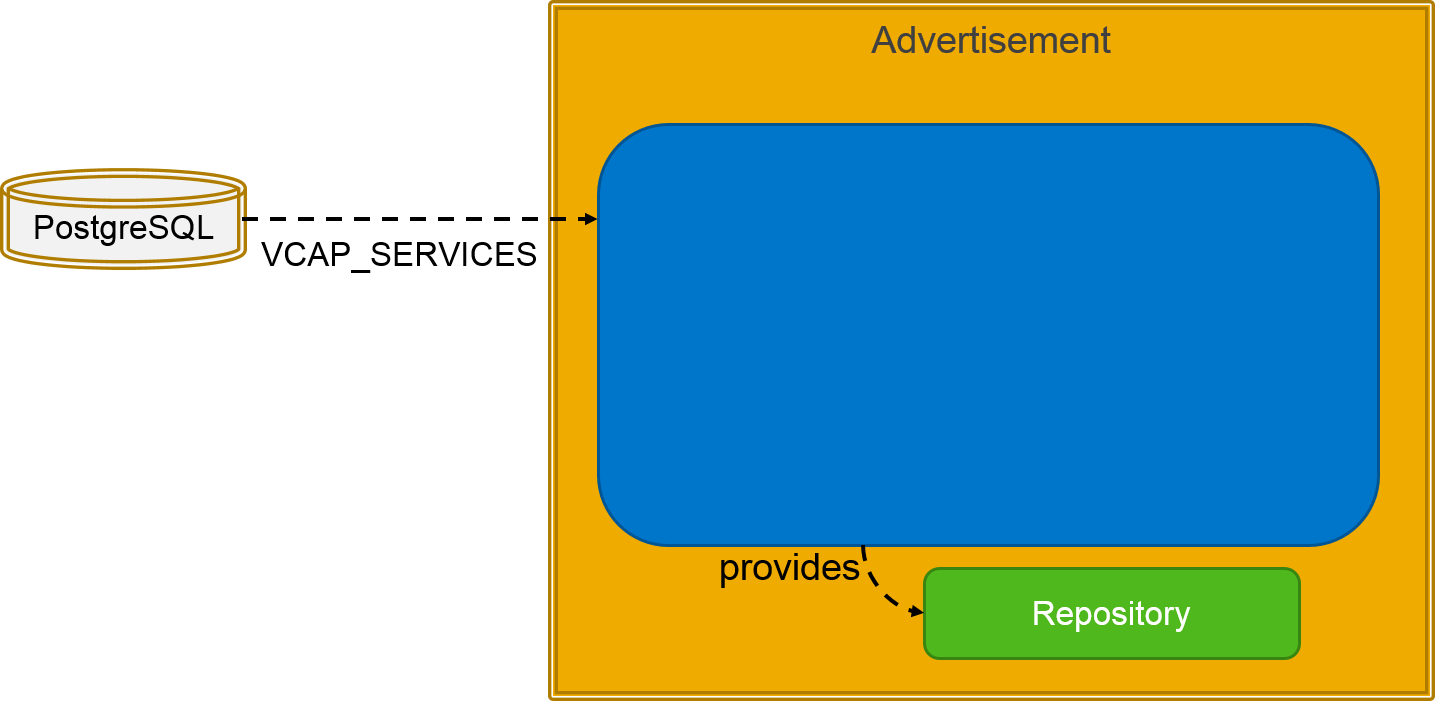
\includegraphics[width=0.9\textwidth]{../Z_ReuseImages/images/DBConnectionSetup_blackbox}
\end{figure}
{
\tiny
The environment variable \codealt{VCAP\_SERVICES} contains cloud database connection information
}
\end{frame}

\begin{frame}{Setup Database Connection}{Flow of Configuration Data}
\begin{figure}
  	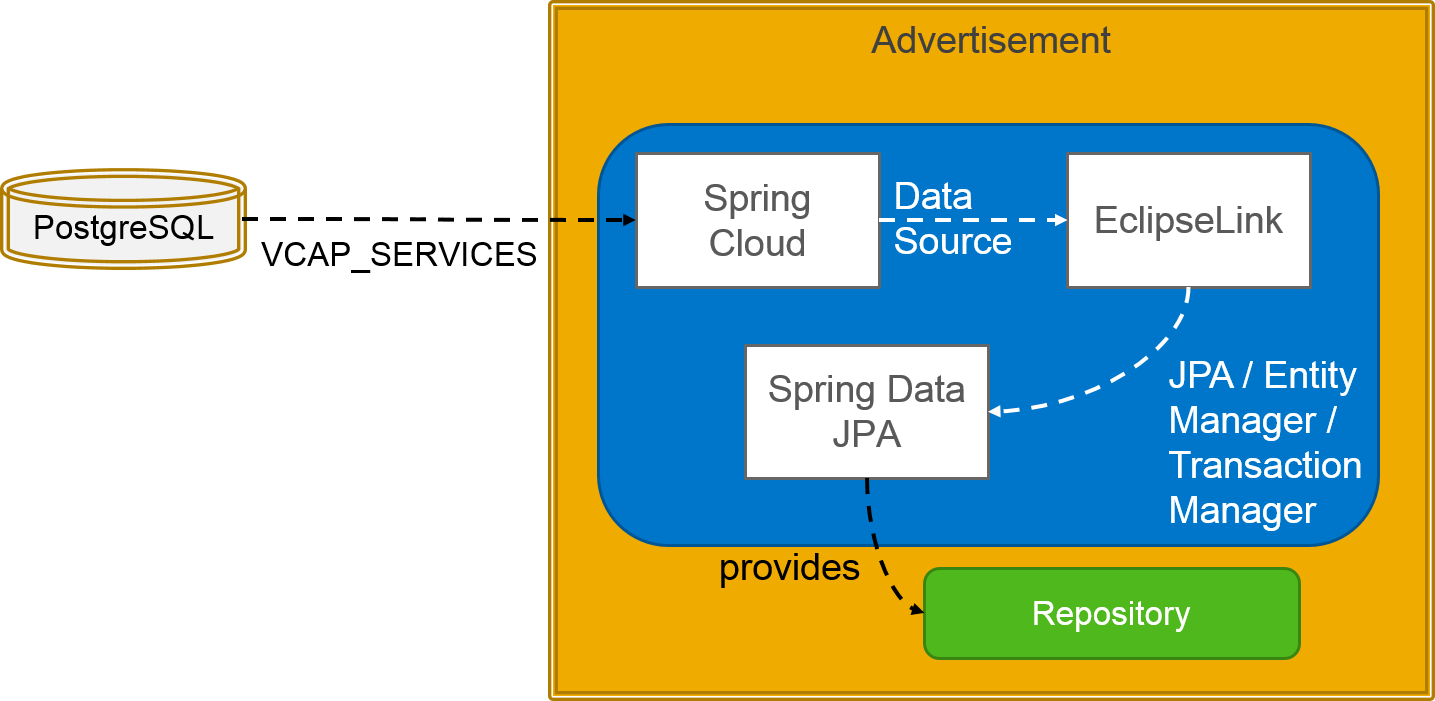
\includegraphics[width=0.9\textwidth]{../Z_ReuseImages/images/DBConnectionSetup}
\end{figure}
{
\tiny
The environment variable \codealt{VCAP\_SERVICES} contains cloud database connection information
}
\end{frame}


\begin{frame}{Exercise 8 (Part 1)}
\begin{figure}
		\includeGraphicsExerciseEightPartOne{width=0.7\textwidth}
	\end{figure}
\colorlink{https://github.com/ccjavadev/cc-coursematerial/blob/master/ConnectDatabase/Exercise_8_Part1_ConfigurePersistence.md}{Exercise 8 (Part 1): Configure Persistence}
\end{frame}

\begin{frame}{Exercise 8 (Part 2)}
\begin{figure}
		\includeGraphicsExerciseEightPartTwo{width=0.7\textwidth}
	\end{figure}
\colorlink{https://github.com/ccjavadev/cc-coursematerial/blob/master/ConnectDatabase/Exercise_8_Part2_UseRepositoryToAccessDatabase.md}{Exercise 8 (Part 2): Use Repository to Access Database}
\end{frame}

\begin{frame}[fragile]{Inject Mocked Beans in (Unit) Test}

\begin{columns}
	\begin{column}[T]{.35\textwidth}
\begin{block}{Application Code}
\begin{lstlisting}
class WebShop {
  @Inject
  private CreditCheck creditCheck;
}
\end{lstlisting}
\end{block}
\end{column}
\begin{column}[T]{.6\textwidth}
\begin{block}{JUnit Test Code}
\begin{lstlisting}[language=Java,belowskip=0mm,aboveskip=0mm]
@RunWith(SpringJUnit4ClassRunner.class)
@ContextConfiguration(classes = TestConfig.class)
public class WebShopTest {
  ...
}

@Configuration
public class TestConfig {
  @Bean
  CreditCheck creditCheck() {
    return Mockito.mock(CreditCheck.class);
  }
}
\end{lstlisting}	
\end{block}
\end{column}
\end{columns}
\begin{itemize}
\item \codealt{@Configuration} annotated Class is a source of \emph{Bean} definitions
\item \codealt{@Bean} annotated Method returns object to be registered in the \\Spring application context
\end{itemize}
\end{frame}


\begin{frame}{Exercise 9 }
\begin{figure}
		\includeGraphicsExerciseNine{width=0.7\textwidth}
	\end{figure}
\colorlink{https://github.com/ccjavadev/cc-coursematerial/blob/master/ConnectDatabase/Exercise_9_ImplementJPAEntity.md}{Exercise 9: Implement JPA Entity test-driven}
\end{frame}

\begin{frame}[fragile]{Backing Services}
\framesubtitle{Create and Connect in Cloud Foundry}
\begin{block}{List available services}
\codealt{\$ cf marketplace}

\tt
\begin{tabular}[h]{lll}
\underline{service} & \underline{plans} & \underline{description} \\
hana            & hdi-shared & HANA in-memory database\\
\alert<2>{postgresql} & \alert<2>{v9.4-dev}       & PostgreSQL database\\
\end{tabular}
\end{block}

\begin{block}<2->{Create service instance (in your space)} 
\codealt{\$ cf create-service \alert<2>{postgresql v9.4-dev} \alert<3>{my-database}}
\end{block}

\begin{block}<3->{Bind service instance (effective after app restart)}
\codealt{\$ cf bind-service my-app \alert<3>{my-database}}\\
\end{block}

\onslide<4->{\alert{Warning:} \codealt{cf delete-service} deletes all database data!}
\end{frame}

\begin{frame}{Using a backing service: \codealt{cf bind-service}}
\begin{center}
	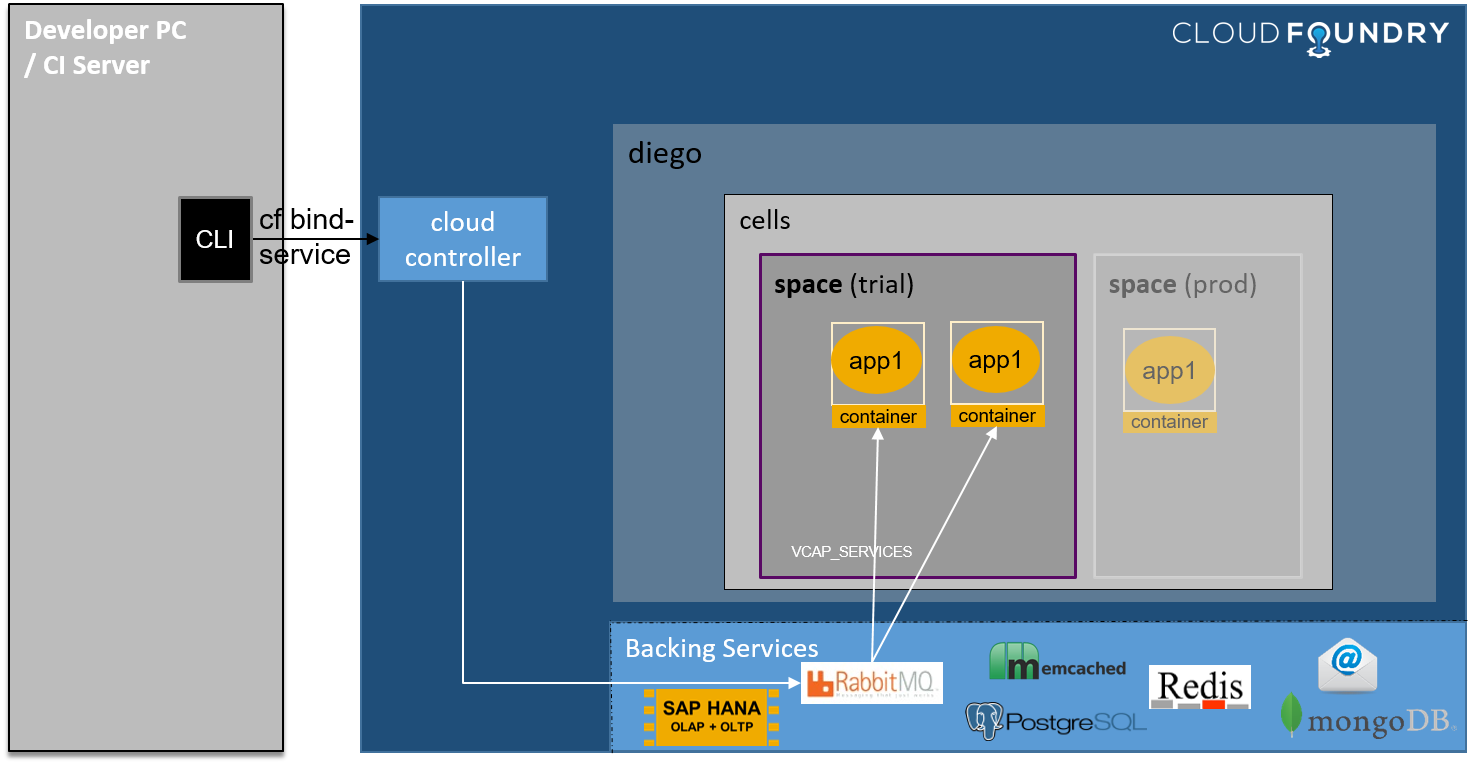
\includegraphics[width=0.9\textwidth]{../ConnectDatabase/images/CF_Basics_7_backing}
\end{center}
\colorlink{http://docs.run.pivotal.io/devguide/services/}{CF Doc - Services Overview}
\end{frame}

\begin{frame}[fragile]{Backing Services}{Usage in Microservice}
By binding a service, Cloud Foundry provides the credentials necessary to connect to the service instance via an \textbf{environment variable}.
\vfill

Example:
\begin{block}{\code{\$ cf env my-app}}
\vspace{-5mm}
\scriptsize
\begin{verbatim}
 "VCAP_SERVICES": {
  "postgresql": [{
    "credentials": {
     "dbname": "random-db-name",
     "hostname": "10.1.2.3",
     "password": "secret-pw",
     "username": "random-user-name"
     [...]
\end{verbatim}
\vspace{-5mm}
\end{block}
\colorlink{http://docs.run.pivotal.io/devguide/deploy-apps/environment-variable.html}{CF Doc - Cloud Foundry Environment Variables}

\end{frame}


\begin{frame}{Exercise 10}
	\begin{figure}
		\includeGraphicsExerciseTen{width=0.8\textwidth}
	\end{figure}
\colorlink{https://github.com/ccjavadev/cc-coursematerial/blob/master/ConnectDatabase/Exercise_10_DeployAdsWithDBServiceOnCF.md}{Exercise 10: Deploy Ads on Cloud Foundry}
\end{frame}


\begin{frame}[fragile]{JPA Custom Query}
\begin{itemize}
\item JP QL is portable across all databases not like native SQL
\item Queries refer to entity class / field names rather than tables and columns
\end{itemize}
\vfill
\uncover<2->{Examples:}
  \begin{itemize}
\begin{visibleenv}<2->
	\item select id from user where city="Berlin"
		\begin{lstlisting}
entityManager.createQuery("SELECT u.id FROM User u WHERE u.city='Berlin'");
		\end{lstlisting}
\end{visibleenv}
\begin{visibleenv}<3->
	\item Typed query with named parameter (to prevent SQL Injection)
	\begin{lstlisting}
String qlString = "SELECT MAX(p.price) FROM PurchaseOrder o
                     JOIN o.lineItems l JOIN l.product p JOIN p.supplier s 
                     WHERE s.name=:parameter";
TypedQuery<Double> query = entityManager.createQuery(qlString, Double.class);
query.setParameter("parameter", supplier);
Double maxPrice = query.getSingleResult();
	\end{lstlisting}

\end{visibleenv}
\end{itemize}

\end{frame}

\begin{frame}[fragile]{Native Queries in JPA}
\begin{itemize}
\item SQL Queries for leveraging database specific functionalities
\item Queries do NOT refer to entity class / field names
\end{itemize}
\vfill
\begin{visibleenv}<2->
HANA DB Examples:
  \begin{itemize}
	\item Exact search
		\begin{lstlisting}
entityManager.createNativeQuery("select * from T where contains(column1, 'dog OR cat');");
		\end{lstlisting}
	\item Freestyle search over multiple columns
		\begin{lstlisting}
entityManager.createNativeQuery("select * from T where CONTAINS( (column1,column2,column3), 'cats OR dogz', FUZZY(0.7));");
		\end{lstlisting}
  \end{itemize}
\end{visibleenv}
\end{frame}

\begin{frame}{[Optional] Exercise 11}
\colorlink{https://github.com/ccjavadev/cc-coursematerial/blob/master/ConnectDatabase/Exercise_11_Develop_Custom_Queries.md}{Exercise 11: Develop Custom Queries}
\end{frame}

\begin{frame}{Database Schema Evolution}
\textbf{NEVER} let JPA \textbf{create and extend} your database schema, as it \ldots
\begin{itemize}
\item applies DDL statements in an implicit and incomprehensible way
\item supports only very basic database schema changes, which results only in naive \codealt{ALTER TABLE} statements
\item is not appropriate for production: high chance that data gets inconsistent or lost
\end{itemize}
\vfill
\visible<2->{
\textbf{Database schema migration tools:}
\begin{itemize}
\item \colorlink{http://www.liquibase.org}{Liquibase}: describe migration in XML, YAML, JSON or SQL; DB independent
\item \colorlink{https://flywaydb.org}{Flyway}: describe migration in SQL; convention over configuration
\end{itemize}
}
\vfill
\colorlink{https://github.wdf.sap.corp/cc-devops-course/coursematerial/blob/master/DevOps/Zero_Downtime_Deployment/Zero-Downtime_Migration.pptx}{Zero-Downtime Migration: Concepts and Examples}
\end{frame}

\begin{frame}[fragile]{Example: Liquibase}
\scriptsize
\begin{block}{changelog-master.xml}
\begin{lstlisting}[language=XML,belowskip=0mm,aboveskip=0mm]
<databaseChangeLog>
...
  <include file="com/sap/bulletinboard/ads/db/changelog-1.0-create-ads-table.xml"/> 
  <include file="com/sap/bulletinboard/ads/db/changelog-1.1-add-version-col.xml"/>  
</databaseChangeLog> 
\end{lstlisting}
\end{block}
\vfill
\begin{block}{changelog-1.1-add-version-col.xml}
\begin{lstlisting}[language=XML,belowskip=0mm,aboveskip=0mm]
<databaseChangeLog>
  <changeSet author="John Doe" id="1.1-add-version-col">
    <addColumn tableName="advertisement">
      <column name="version" type="BIGINT" value="42"/>
    </addColumn>
  </changeSet>
</databaseChangeLog>
\end{lstlisting}
\end{block}
\small
\colorlink{https://github.com/ccjavadev/cc-coursematerial/blob/master/ConnectDatabase/DatabaseSchemaEvolution.md}{Detail Notes}
\\\colorlink{http://databaserefactoring.com}{Collection of Database Refactoring Patterns}
\end{frame}

\begin{frame}[fragile]{Demo: Create Hana artefacts via HDI}
\begin{figure}
  	\includeGraphicsExerciseHANAHDI{width=0.93\textheight}
\end{figure}
\colorlink{https://github.com/ccjavadev/cc-coursematerial/blob/master/Hana/Demo_HANA_HDI.md}{HANA HDI Exercise: Create Hana artefacts via HDI}
\end{frame}


\begin{frame}{Further Learning Opportunities}
\textbf{E-Learning}
	\begin{itemize}
	\item \colorlink{https://github.wdf.sap.corp/cloud-native-dev/java-persistence/wiki}{Efficient Java Persistence with JPA}
	\end{itemize}
\vfill
\textbf{Recommended Books}\\

\includegraphics[height=24mm]{../ConnectDatabase/images/ProJPA_2Edition}   
\hspace{3mm}

\includegraphics[height=24mm]{../ConnectDatabase/images/HighPerformanceJavaPersistence}

\end{frame}

